\chapter{Developer documentation}
\label{ch:impl}

For this project a high level programming language was needed which can support dynamic typing for creating easy statements and storing
lot of different data, the language also has to support runtime interpretation so the user defined statements can be used without
creating a whole new programming language and compiler for it. For these reasons JavaScript with the node.js runtime was chosen. 

\newpage

\section{Architectural Overview}

The toolkit is heavily depends on the libgit2 \cite{libgit2} library which is a portable, pure C implementation  if the Git core methods,
this library has a version for JavaScript and Node.js which is the nodegit\cite{nodegit}.
The whole toolkit architecture can be represented with the following diagram:

\begin{figure}[H]
	\centering
	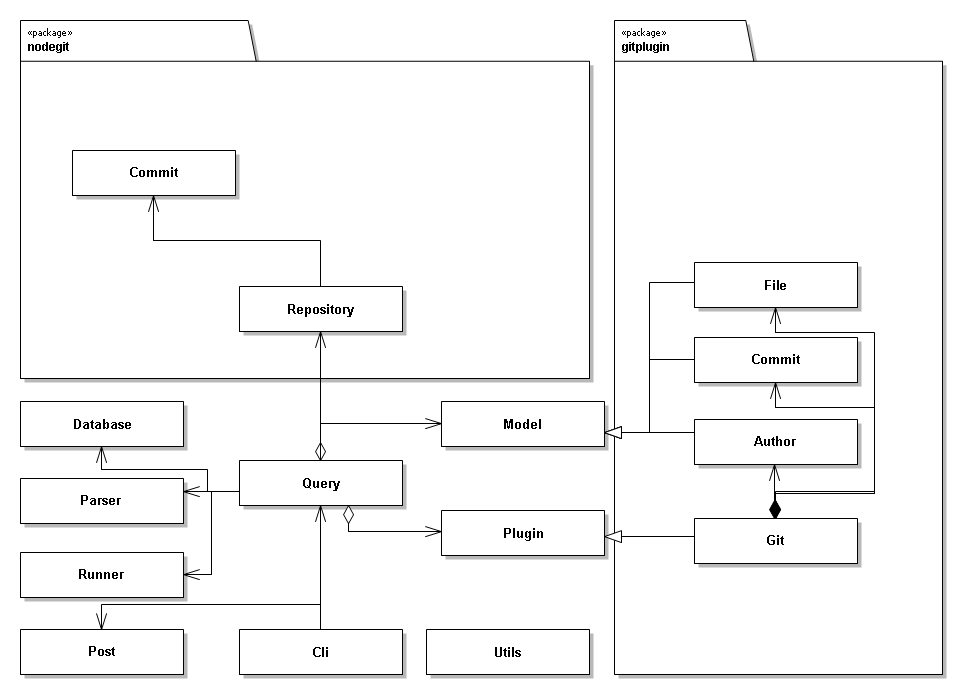
\includegraphics[width=350px]{uml}
	\caption{UML diagram of the toolkit}
	\label{fig:fig-help}
\end{figure}

The \textit{Query} class is responsible to connect all the modules altogether and also for the IO operations. The query also also
responsible for reading the history from the repository and passing it to the plugins for parsing. The parse data will be stored
in the \textit{Database}. Before the parsing happens the input script also has to be recognized which is done by the \textit{Parse}
module. After both of them is ready the \textit{Runner} module will run the query based on the script and database.
\newpage

\subsection{Database}

We need to somehow store all the data coming from the parser and plugins. We can assume that the plugins will reduce the size of the
pure data from the repository history. So to provide maximum performance for the query we can use an in-memory database. 
We can also assume that the database will be immutable after the parsing is done. 

The database is collections of hash maps based on the models. The hash map keys are defined by its model \textit{key()} method.
The reason behind this database structure is in the join mechanism in the query. The hash map is implemented with the built in 
\textit{Map}\cite{map} in JavaScript which has access to a given key by a time and space complexity of:

\( O(1) \)

In this way if we connect two models where at least of the models field is a key then we can assume that:\newline
If: N is the count of records by the A model, M  is the count of records by the B model. Then:
	
\[O(N * M) \Leftrightarrow O(N * 1) \Leftrightarrow O(N)\]

\begin{figure}[H]
	\centering
	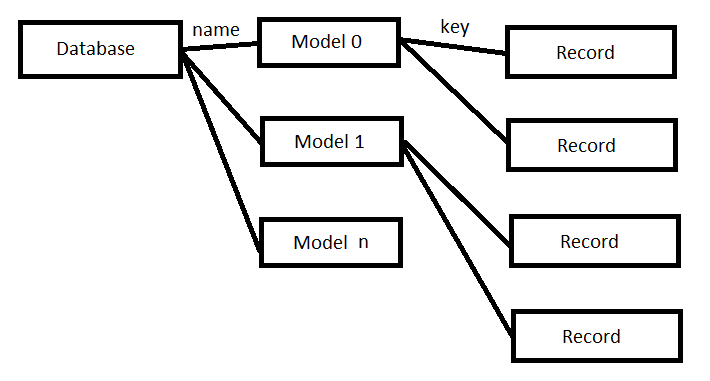
\includegraphics[width=350px]{database}
	\caption{Structure of the database}
	\label{fig:fig-help}
\end{figure}
\newpage

\subsection{Extensions}

As discussed in the Extending with plugins are the way to add more features to extensions to the toolkit.
Let's look at the included basic \textbf{Git} plugin and its models \textbf{Commit}, \textbf{Author}, \textbf{File}.
This plugin will do the most basic parsing for the histroy which is to extract the commits, the authors, and the files
in the project.

What is needed to make a plugin:
\begin{itemize}
	\item \textit{init()} - The init will be called when repository is opened.
	\item \textit{parse(db, commit)} - This will be called for each commit, the database is expossed as a \textbf{Observer pattern}
	\item \textit{post()} - This will be called when all the commits are parsed
\end{itemize}

The commit in the \textit{parse(db, commit)} is defined in the libgit2 plugin.

The plugin also provided information about itself and what models brings to the database. 
The models will be loaded into database before \textit{init()} is called.

\subsubsection{Functions}

Functions are help for the user to predefined some often used functions for the given plugin.
For example: we may only need a short id for the commit so we can call \textit{short(sha)} inside our query expressions.
Behind the scene this will be injected into the sandbox where the expressions are evaluated.

To define a new functions just pass the function in an array in the \textit{functions()} method.

\subsubsection{Reductors}

Reductors are similar to Functions but its only can be used if a grouping is presented in the query. This will
run for each record in that group. The reductor should be a function and has 2 parameter \textit{reductor(acc, obj)}.
The \textit{acc} will accumulate the result and the object will be the record itself.

To define a new reductor just pass the function in an array in the \textit{reductors()} method.

\subsubsection{Model}

A model is simply defining the structure of data it has two major function \textit{parse(input)}, \textit{parse(key)}. 
This will take the input and transform it that way the database is storing them. 
\textit{name()} will be the name how it can be refereed in the from tag.

Lets look at the Git plugin:

\lstinputlisting[caption={plugins/git.js}]{../plugins/git.js}

\subsection{Parsing and validating scripts}

The one of the most important step is properly read and process the input
from the user script file. Storing this data in the right structure is a key
to speed up the process of the parsing and running the query.

The input script file is a YAML\cite{yaml} which is a human readable data-serialization language. Because the script file structure is declarative
this markup language is ideal. The actual parsing of the YAML file is done by
a third party library from npm which is the yaml\cite{yaml-pck} package.

After parsing the input file into a JavaScript Object the real parsing begin: 

The core tags of script file are the \textit{From}, \textit{Select}, \textit{Where}, all of them is required.
\newpage
\subsection{From}
The used models should be enumerated here and separated with a \textit{;} character. The parser will create an Object in the \textit{Query} which will map each rename to a model.

 \begin{figure}[H]
 	\centering
 	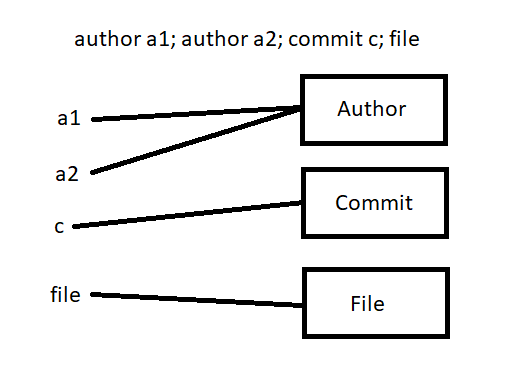
\includegraphics[width=350px]{fromconn}
 	\caption{Structure of the parsed From tag}
 	\label{fig:fig-help}
 \end{figure}

\subsection{Select}
Here the selected \textit{model.field} should be provided with a \textit{;} 
separator character. The \textit{\$} wildcard can be used to select all the
available fields. This can be mixed with a custom transformation of a field.

Here JavaScript statements can be provided which will be evaluated when the
Query runner stops. The statement is transformed by these rules:

\begin{itemize}
	\item If a model with a field is present it will be replaced with a special expression: \textbf{\_\_o['model.field']}
	\item If a plugin provided function is present it will be replaced with: \textbf{\_\_f.function(args)}
	\item If a plugin provided reductor is present it will be replaced with: \textbf{\_\_r.reductor(args)}
\end{itemize}

You can provide multiple field for one selection but you can add without any of it. The header of the selection
will be always the provided statement.

The transformation of the statement is needed because later on when \textit{Runner} start to process the script
it will transform each and every JavaScript statement into a function by:

Creating a lambda expression of the statement: 

 model.field + 2 + fun(4)\newline 
 To:\newline
 (\_\_o, \_\_f) => \{ return \_\_o['model.field'] + 2 + \_\_f.fun(4) \}\newline

This can be cached into the memory so when it has to be evaluated for each record this can speed up the process.

The same principles applies for all the JavaScript statements in the input file, only the \textit{Where} tag makes an exception. 

Note: The JavaScript will be executed in a sandbox mode no node.js module is
available. 

\newpage
\subsubsection{Where}

In the where tag two parsing is happening: The join and where. Both the where and join are part of the \textit{Runner} workflow. Lets look at this statement, where we are using the the following models: commit c1, commit c2, commit c3

\[ c1.sha ==\ '5b2c7'\ \&\&\ c2.sha == c1.sha\ \&\&\ c3.sha == c1.sha\]

Now lets convert this statement into a logic expression where we want to specify the required
data set:

\[( \forall{c1}\forall{c2}\forall{c3}(c1.sha ==\ '5b2c7' \wedge c2.sha == c1.sha \wedge c3.sha == c1.sha)\]

Lets simply the expression by:

\[ \forall{c1}(c1.sha ==\ '5b2c7') \wedge \forall{c1}\forall{c2}(c2.sha == c1.sha) \wedge \forall{c1}\forall{c3}(c3.sha == c1.sha)\]

Now lets replace the universal quantifier with predicates and we get:

\[ P1(c1) \wedge P2(c1,c2) \wedge P3(c1,c3)\]

In this way we can break up the expression into smaller pieces so the parts can be evaluated without the fully fledged record. This will be important later on...

Before we parse the \textit{Where} flag we are replacing the joins with placeholders.
As discussed in the User Documentation if one of the \textit{model.field} is a key then
we can make faster the \textit{Runner} by using the Maps in the \textit{Database}.

We can assume that all the joins will be done during the run so we can replace these with a
\textbf{true} expression. The join will be stored in a special Object in the Query which will
be used by the \textit{Runner} itself.

\newpage
\subsection{Parsing Git histroy}

Before talking about how the history is evaluated into a user readable output. Lets take a look
how the history parsing. This part is done by the main \textit{Query} class with the loaded
plugin. First the repository is loaded either by cloning it from Github or by loading a local copy of it. After that if the script file contain the main commit sha then the commit will be the starting point of the algorithm if not them the master commit will provide the starting point.

The history walker algorithm is based on a breadth-first search.

\begin{algorithm}[H]
	\caption{History walker} 
	\label{alg:ibb} 
	\textbf{\underline{function}} load($Plugins$ ,$Repository, commit$)
	\begin{algorithmic}[1] % display line numbers before every n line, here n = 1
		\For{all $plugin$ in $Plugins$}
		\State plugin.setup()
		\EndFor
		\State let Q be a queue
		\State label commit as explored
		\State Q.enqueue(commit)
		\While{( ${\cal Q}$\ is\ not\ empty )}
		\State $c$ := $Q$.dequeue()
		\For{all edges from $v$ to $w$ in $Repository$.parents($v$)}
		\If{$w$ w is not labeled as explored }
		\State label w as explored  
		\State Q.enqueue(w) 
		\For{all $plugin$ in $Plugins$}
		\State plugin.fetch($w$)
		\EndFor 
		\EndIf
		\EndFor
		\EndWhile
		\For{all $plugin$ in $Plugins$}
		\State plugin.post()
		\EndFor
		\end{algorithmic}
\end{algorithm}

After finishing the parsing the Database is locked and can be considered as an immutable object. 

\newpage

\subsection{Running the query}

The most important part of the project is how we can efficiently query in the parsed data. At this point we have a in-memory database where we can search in \(O(1)\) time, we were able break up the \textit{Where} statement into smaller predicates.

The goal is to join all the tables together and filter out the rerecords where the condition does not met.

\subsubsection{Trivial solution problem}
The most trivial solution is to connect all models together and run the full \textit{Where} statement on the fully fledged record. This can work in most of the cases but if we want to run it on a big repository then we will end up running out of memory quickly. For example lets look at this:

Let: $commit.count$ = 50 = $N$

if we would like to join the commit model in $M$ times we would end up in a time and space complexity of:

\[ O(N_1 * N_2 * \dots * N_M ) \Leftrightarrow O(N^M) \]

Lets assume that the heap memory limit in node.js with 8G of allocated memory is around $~10.000.000$ records. So in this way we are limited by

\begin{table}[H]
	\centering
	\begin{tabular}{ | m{0.25\textwidth} | m{0.35\textwidth} | m{0.15\textwidth} | }
		\hline
		\textbf{N} & \textbf{Joined records count} & \textbf{Under memory limit} \\
		\hline \hline
		\emph{1} & 50 & $\checkmark$ \\
		\hline
		\emph{2} & 2.500 & $\checkmark$ \\
		\hline
		\emph{3} & 125.000 & $\checkmark$ \\
		\hline
		\emph{4} & 6.250.000 & $\checkmark$ \\
		\hline
		\emph{5} & 312.500.000 & $\times$ \\
		\hline
		\emph{$\infty$} & $\dots$ & $\times$ \\
		\hline
	\end{tabular}
	\caption{Time and space analysis on trivial join}
	\label{tab:tsj-1}
\end{table}

As we can see even for a small repository a 5 way join is cause out of memory problems. But if we take into consideration that a large repository with $10.000$ commits, even a 2 way join can cause problems which is not acceptable. 
\newpage

\subsubsection{Solution}

Lets assume first that the user is provided "useful" query script which means the result of the query should be human readable data size. With some trick we can reduce the size of the fully fledged dateset without losing any information or by giving up flexibly of the query language. 

\subsubsection{Predicates}

As discussed in the \textit{Where} tag parsing we are break up the whole statement into pieces. Let's take a look on the previous example:

\[ P1(c1) \wedge P2(c1,c2) \wedge P3(c1,c3)\]

This means we have 3 separated predicate where the parameters are the model dependencies, this means we can create a dependency graph by filtering with this predicates as soon as possible  in the execution tree (Circles are joins).

 \begin{figure}[H]
	\centering
	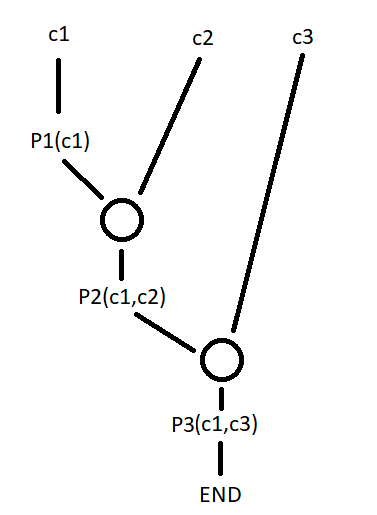
\includegraphics[width=250px]{exectree}
	\caption{Execution tree (Top to down)}
	\label{fig:fig-elist}
\end{figure}

\newpage

Currently the toolkit is single threaded application so there is no optimization with the execution by doing the filtering and joins parallel.

Because of that we can convert the execution tree into an execution list by doing the predicates as soon as possible in the execution order.

 \begin{figure}[H]
	\centering
	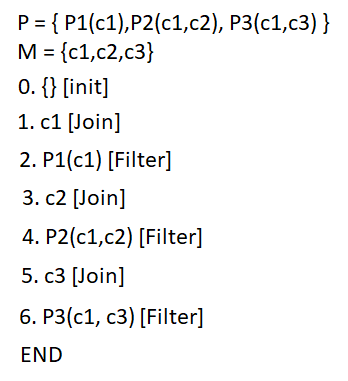
\includegraphics[width=250px]{execlist}
	\caption{Execution list}
	\label{fig:fig-liste}
\end{figure}

The predicates are ordered by how many parameters it have if the same the order which they were given in the script file will be take into consideration. The only exception if a join on is present.

\newpage
\subsubsection{Join on}
As discussed in the user documentation join-on section the join-ons will be removed from the statement and handled separately. Lets look at how this effect the \textbf{Runner} execution list. This step can be done because the structure of the database.

If a join can be done with join-on it will be preferred in that way if the predicate requires the model which can be join-on then the join-on dependency will be joined first. Lets look on an other execution tree:

 \begin{figure}[H]
	\centering
	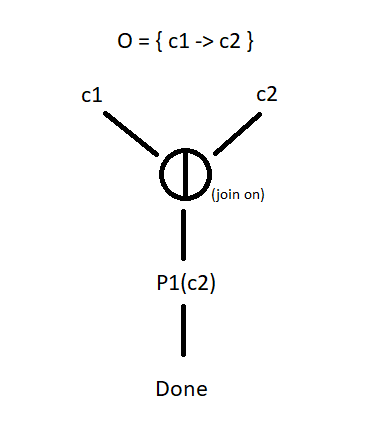
\includegraphics[width=250px]{exectree-join}
	\caption{Execution tree with join-on (Top to down)}
	\label{fig:fig-tree}
\end{figure}

And the execution list will be:

\begin{figure}[H]
	\centering
	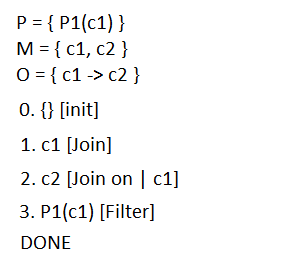
\includegraphics[width=150px]{execlist-join}
	\caption{Execution list with join}
	\label{fig:fig-joine}
\end{figure}

\section{Tools}

The development of the toolkit requires to use special tools to make the it easy and fast. The creation of the software is mostly done in windows but for each release a manual test is done in Linux too.

\subsection{Visual Studio Code}

Visual Studio Code is a streamlined code editor with support for development operations like debugging, task running, and version control. It aims to provide just the tools a developer needs for a quick code-build-debug cycle and leaves more complex workflows to fuller featured IDEs, such as Visual Studio IDE\cite{vscode}

It has build in support for JavaScript syntax, has an easy to use file system navigator and the built in terminal helped a lot to test the whole toolkit in only one application. Also has a built in Git tool so it can be used as a Git client too.

\begin{figure}[H]
	\centering
	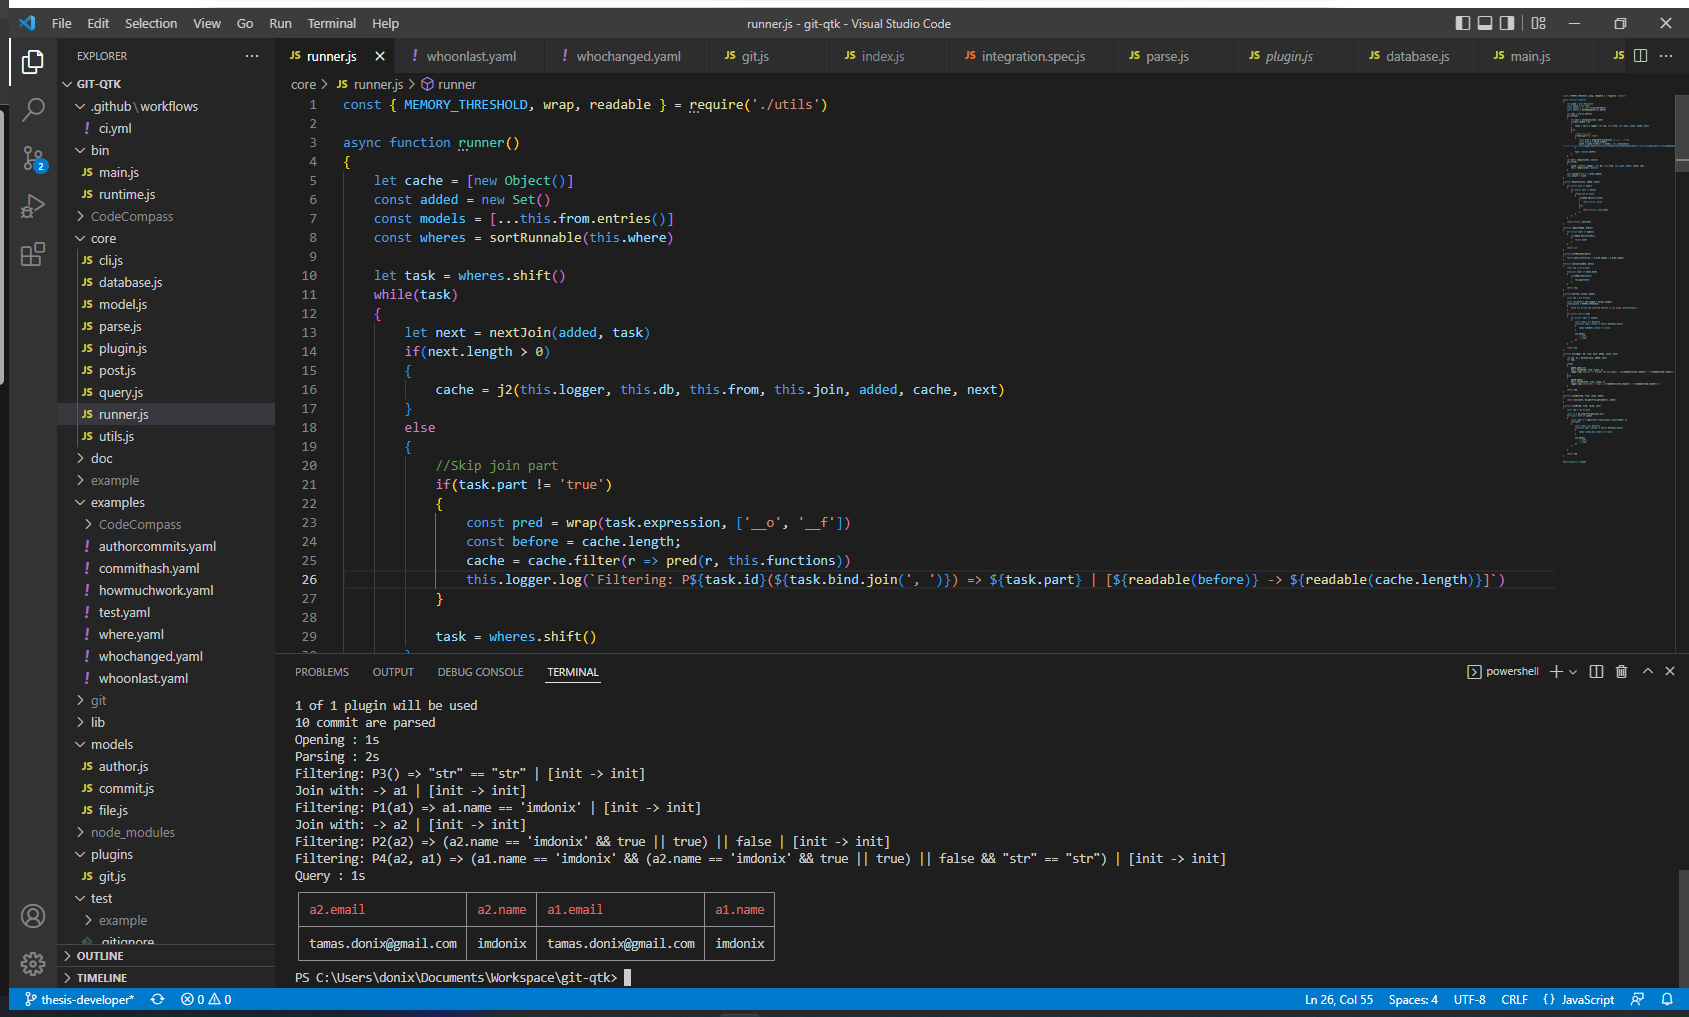
\includegraphics[width=400px]{vscode}
	\caption{Project in Visual Studio Code}
	\label{fig:fig-studio}
\end{figure}

\newpage
\subsection{Github}

GitHub is a provider of Internet hosting for software development and version control using Git. It offers the distributed version control and source code management (SCM) functionality of Git, plus its own features. It provides access control and several collaboration features such as bug tracking, feature requests, task management, continuous integration, and wikis for every project.\cite{gitbib}

\begin{figure}[H]
	\centering
	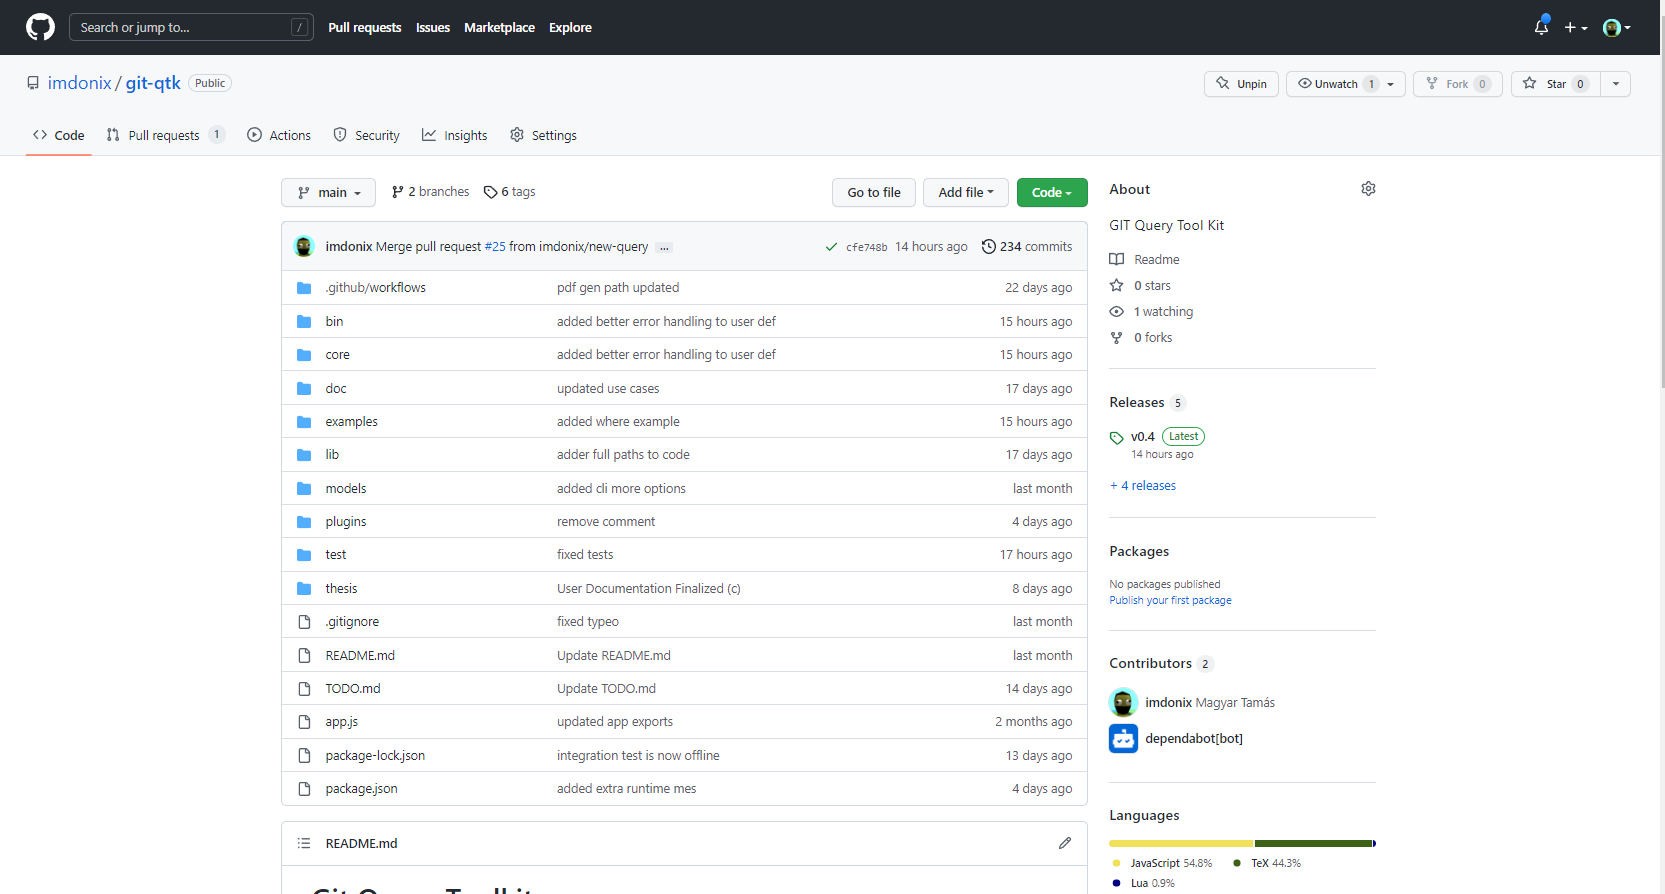
\includegraphics[width=400px]{github}
	\caption{Github page of the project}
	\label{fig:fig-github}
\end{figure}

It way obvious to host the project on Github, because it can be also an input repository for the toolkit. The whole project is under version control and with the help of pull requests I was able to track my work easily. By creating feature or bug issues I was able to work on the project effectively.

\newpage
\subsection{Continues integration}

With the help of GitHub Actions the project was under continues integration which runs the tests for each and every commit and also create a runtime measurement report as artifact. 
The thesis document itself is version controlled on Github and generated for each push. 

\begin{figure}[H]
	\centering
	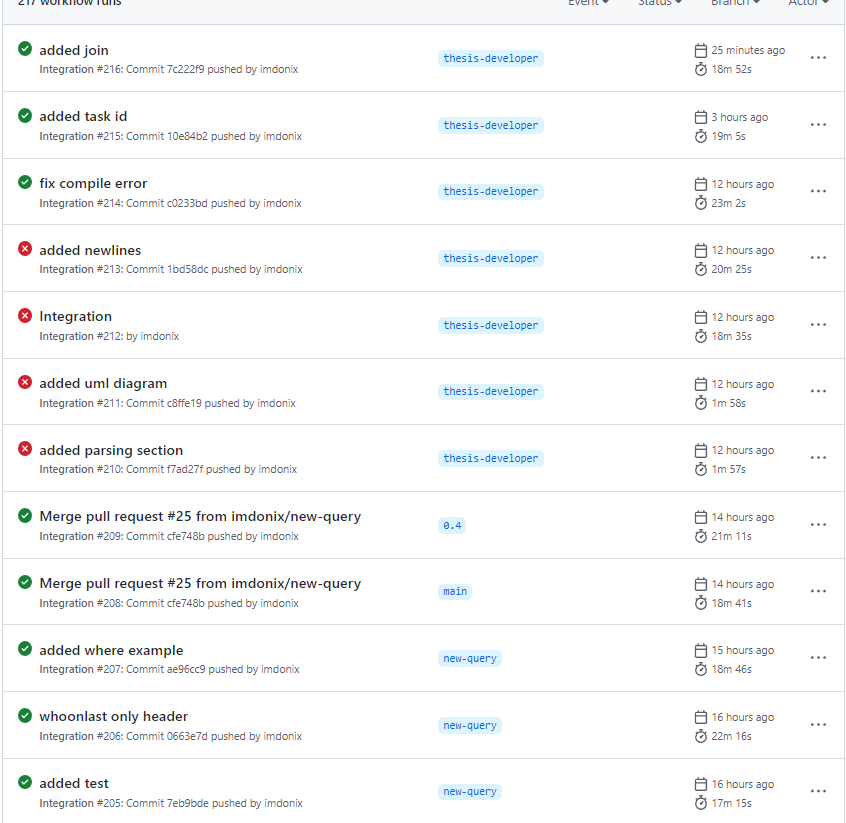
\includegraphics[width=400px]{action}
	\caption{Github Actions}
	\label{fig:fig-act}
\end{figure}


\begin{figure}[H]
	\centering
	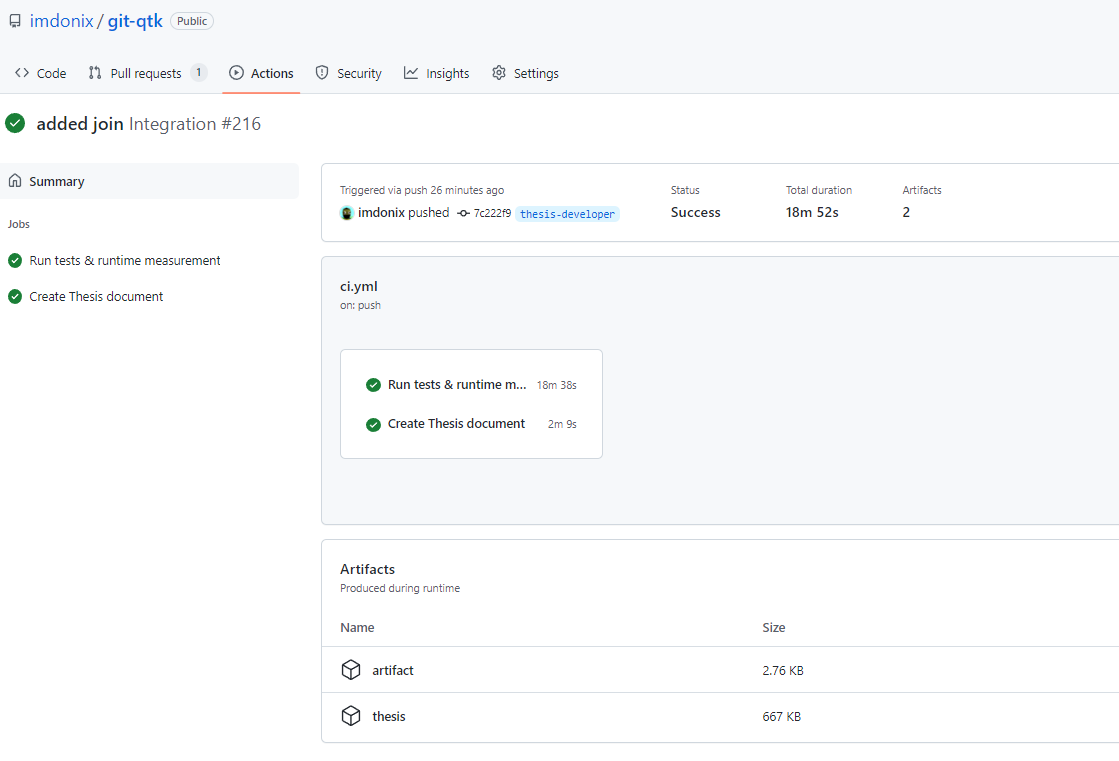
\includegraphics[width=400px]{run}
	\caption{Github Actions - Integration}
	\label{fig:fig-int}
\end{figure}


\section{Testing}

For testing each module in this complex toolkit tests where created to provide stability. The testing is done with the mocha.js\cite{mocha} node.js package. Which is a feature-rich JavaScript test framework running on Node.js and in the browser, making asynchronous testing simple and fun. Mocha tests run serially, allowing for flexible and accurate reporting, while mapping uncaught exceptions to the correct test cases.

\begin{figure}[H]
	\centering
	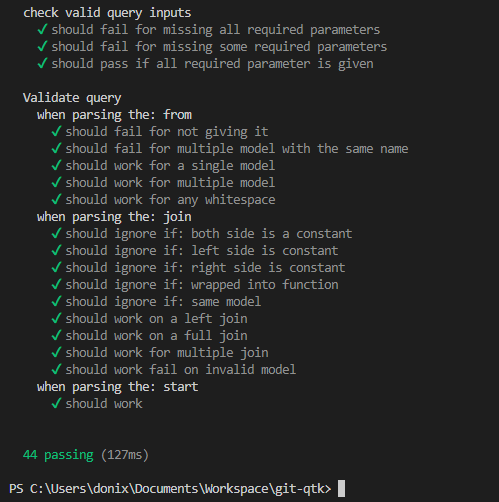
\includegraphics[width=350px]{test}
	\caption{Tests}
	\label{fig:fig-test}
\end{figure}

\subsection{Unit tests}

Unit tests are created for each module of the toolkit:

\begin{itemize}
	\item Parsing: From (9)
	\item Parsing: Select (6)
	\item Parsing: Where (5)
	\item Parsing: Limit (4)
	\item Parsing: Order (5)
	\item Parsing: Join (9)
	\item Parsing: Start (1)
	\item CLI (3)
\end{itemize}

A total of 41 unit test are added to the project. These are mostly black box testes but some white box test also present.

\subsection{Integration tests}

During the development integration tests was a big help to get information about the health of the tool. This contains a simple test on a prepackaged small repository repository for only validating the result of the toolkit.

So when a optimization change is made in a module I was able to validate how its working in real life.

The integration test unzip the sample repository and run the query on it then its checking the following values:

\begin{itemize}
	\item Are the plugins run correctly?
	\item Is the required models present in the database?
	\item Is the records in the database are valid?
	\item Is the output of the tool are same as the expected?
\end{itemize}

\subsubsection{How to run the tests}

To run the tests just run the following command:

\[ npm\ test \]


\chapter{Runtime measurement}
\label{appx:simulation}

An important requirement for the toolkit to be efficient and able to handle large repositories. This is done by the optimizations in the history parser and in the Runner. During the development is was important to track how a change effect the runtime in different script-repository runs.   

For this reason a special action is induced in the toolkit which called runtime measurement. By running it we can get a full report of how much time it takes to run the toolkit on repositories.

The list of bench repository are provided manually and the example script files are used in the process.

\begin{figure}[H]
	\centering
	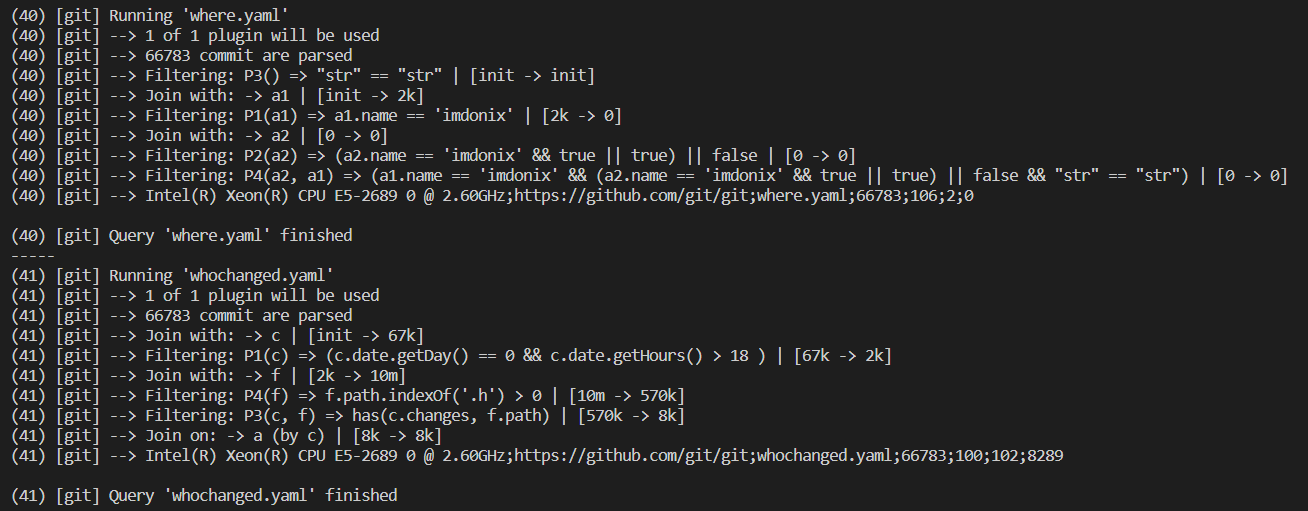
\includegraphics[width=400px]{runtime}
	\caption{Tests}
	\label{fig:fig-runtime}
\end{figure}

\subsubsection{Bench repositories}

\begin{table}[H]
	\centering
	\begin{tabular}{ | m{0.35\textwidth} | m{0.35\textwidth} | }
		\hline
		\textbf{Repository} & \textbf{Commits} \\
		\hline \hline
		\href{https://github.com/imdonix/example}{imdonix/example} & 10 \\
		\hline
		\href{https://github.com/Ericsson/CodeCompass}{Ericsson/CodeCompass} & 905 \\
		\hline
		\href{https://github.com/catchorg/Catch2}{catchorg/Catch2} & 4.044 \\
		\hline
		\href{https://github.com/vlang/v}{vlang/v} & 13.140 \\
		\hline
		\href{https://github.com/git/git}{git/git} & 66.783 \\
		\hline
	\end{tabular}
	\caption{Bench repositories with commit count (On master branch)}
	\label{tab:runtime}
\end{table}

The test run all the example script for all the bench repositories and collect the timed steps into a csv file in the root of the project. If a test fails the error will be printed out instead.

To run the runtime measurement type:
\[npm\ run\ runtime\]

\subsubsection{Test devices}

\begin{table}[H]
	\centering
	\begin{tabular}{ | m{0.15\textwidth} | m{0.5\textwidth} | m{0.13\textwidth} |  m{0.15\textwidth} | }
		\hline
		\textbf{Nickname} & \textbf{CPU} & \textbf{Memory} & \textbf{OS}  \\
		\hline \hline
		Workstation & Intel™ Xeon™ E5-2678 v3 @ 2.50GHz (8c/16t) & 32GB DDR3 1333Mhz  & Windows \\ 
		\hline
		Laptop & AMD Ryzen™ 5 5500U @ 2.1GHz (6c/12t) & 16GB DDR4 2666Mhz & Windows \\
		\hline
		Action & Intel™ Xeon™ 8370C CPU @ 2.80GHz (2c/2t) & 8GB DDR4 3200Mhz & Linux \\
		\hline
	\end{tabular}
	\caption{Bench devices}
	\label{tab:devices}
\end{table}

Note that the GitHub Action provided runner is in a virtual environment so can't use it as a "pure" input for measurement but we can filter out problems which hardly impact the runtime.   

\subsubsection{Results}

\begin{table}[H]
	\centering
	\begin{tabular}{ | m{0.15\textwidth} | m{0.16\textwidth} | m{0.25\textwidth} | m{0.1\textwidth} | m{0.1\textwidth} | m{0.1\textwidth} | }
		\hline
		\textbf{Device} & \textbf{Repository} & \textbf{Script} & \textbf{Parsing} & \textbf{Query} & \textbf{Size} \\ 
		\hline \hline
		Workstation & Catch2 & authorcommits.yaml & 3 s & 1 s & < 1k \\ 
		\hline
		Laptop & Catch2 & authorcommits.yaml & 2 s & 1 s & < 1k \\ 
		\hline
		Action & Catch2 & authorcommits.yaml & 2 s & 1 s & < 1k \\ 
		\hline
		Workstation & Catch2 & commithash.yaml & 4 s & 2 s & ~4k \\ 
		\hline
		Laptop & Catch2 & commithash.yaml & 2 s & 2 s & ~4k \\ 
		\hline
		Action & Catch2 & commithash.yaml & 4 s & 2 s & ~4k \\ 
		\hline
		Workstation & Catch2 & howmuchwork.yaml & 4 s & 2 s & ~4k \\ 
		\hline
		Laptop & Catch2 & howmuchwork.yaml & 2 s & 2 s & ~4k \\ 
		\hline
		Action & Catch2 & howmuchwork.yaml & 4 s & 2 s & ~4k \\ 
		\hline
		Workstation & Catch2 & test.yaml & 3 s & 2 s & ~4k \\ 
		\hline
		Laptop & Catch2 & test.yaml & 3 s & 2 s & ~4k \\ 
		\hline
		Action & Catch2 & test.yaml & 4 s & 2 s & ~4k \\ 
		\hline
		Workstation & Catch2 & where.yaml & 4 s & 2 s & < 1k \\ 
		\hline
		Laptop & Catch2 & where.yaml & 3 s & 2 s & < 1k \\ 
		\hline
		Action & Catch2 & where.yaml & 3 s & 2 s & < 1k \\ 
		\hline
		Workstation & Catch2 & whochanged.yaml & 3 s & 4 s & < 1k \\ 
		\hline
		Laptop & Catch2 & whochanged.yaml & 1 s & 2 s & < 1k \\ 
		\hline
		Action & Catch2 & whochanged.yaml & 4 s & 3 s & < 1k \\ 
		\hline
		Workstation & Catch2 & whoonlast.yaml & 3 s & 1 s & < 1k \\ 
		\hline
		Laptop & Catch2 & whoonlast.yaml & 2 s & 1 s & < 1k \\ 
		\hline
		Action & Catch2 & whoonlast.yaml & 3 s & 1 s & < 1k \\ 
		\hline
		Workstation & CodeCompass & authorcommits.yaml & 2 s & 1 s & < 1k \\ 
		\hline
		Laptop & CodeCompass & authorcommits.yaml & 1 s & 1 s & < 1k \\ 
		\hline
		Action & CodeCompass & authorcommits.yaml & 2 s & 1 s & < 1k \\ 
		\hline
		Workstation & CodeCompass & commithash.yaml & 3 s & 2 s & < 1k \\ 
		\hline
		Laptop & CodeCompass & commithash.yaml & 2 s & 2 s & < 1k \\ 
		\hline
		Action & CodeCompass & commithash.yaml & 2 s & 2 s & < 1k \\ 
		\hline
		Workstation & CodeCompass & howmuchwork.yaml & 3 s & 2 s & < 1k \\ 
		\hline
		Laptop & CodeCompass & howmuchwork.yaml & 2 s & 2 s & < 1k \\ 
		\hline
		Action & CodeCompass & howmuchwork.yaml & 3 s & 2 s & < 1k \\ 
		\hline
		Workstation & CodeCompass & test.yaml & 3 s & 2 s & < 1k \\ 
		\hline
		Laptop & CodeCompass & test.yaml & 2 s & 2 s & < 1k \\ 
		\hline
		Action & CodeCompass & test.yaml & 3 s & 2 s & < 1k \\ 
		\hline
		Workstation & CodeCompass & where.yaml & 1 s & 1 s & < 1k \\ 
		\hline
		Laptop & CodeCompass & where.yaml & 2 s & 1 s & < 1k \\ 
		\hline
		Action & CodeCompass & where.yaml & 2 s & 0 s & < 1k \\ 
		\hline
		Workstation & CodeCompass & whochanged.yaml & 1 s & 1 s & < 1k \\ 
		\hline
	\end{tabular}
	\caption{Runtime measurement - Page 1.}
	\label{tab:mes-2}
\end{table}

\begin{table}[H]
	\centering
	\begin{tabular}{ | m{0.15\textwidth} | m{0.16\textwidth} | m{0.25\textwidth} | m{0.1\textwidth} | m{0.1\textwidth} | m{0.1\textwidth} | }
		\hline
		\textbf{Device} & \textbf{Repository} & \textbf{Script} & \textbf{Parsing} & \textbf{Query} & \textbf{Size} \\ 
		\hline \hline
		Laptop & CodeCompass & whochanged.yaml & 1 s & 1 s & < 1k \\ 
		\hline
		Action & CodeCompass & whochanged.yaml & 2 s & 2 s & < 1k \\ 
		\hline
		Workstation & CodeCompass & whoonlast.yaml & 2 s & 2 s & < 1k \\ 
		\hline
		Laptop & CodeCompass & whoonlast.yaml & 2 s & 1 s & < 1k \\ 
		\hline
		Action & CodeCompass & whoonlast.yaml & 2 s & 1 s & < 1k \\ 
		\hline
		Workstation & git & authorcommits.yaml & 96 s & 1 s & < 1k \\ 
		\hline
		Laptop & git & authorcommits.yaml & 53 s & 1 s & < 1k \\ 
		\hline
		Action & git & authorcommits.yaml & 136 s & 1 s & < 1k \\ 
		\hline
		Workstation & git & commithash.yaml & 98 s & 2 s & ~67k \\ 
		\hline
		Laptop & git & commithash.yaml & 54 s & 2 s & ~67k \\ 
		\hline
		Action & git & commithash.yaml & 138 s & 2 s & ~67k \\ 
		\hline
		Workstation & git & howmuchwork.yaml & 104 s & 2 s & ~67k \\ 
		\hline
		Laptop & git & howmuchwork.yaml & 64 s & 2 s & ~67k \\ 
		\hline
		Action & git & howmuchwork.yaml & 139 s & 2 s & ~67k \\ 
		\hline
		Workstation & git & test.yaml & 108 s & 2 s & ~67k \\ 
		\hline
		Laptop & git & test.yaml & 59 s & 2 s & ~67k \\ 
		\hline
		Action & git & test.yaml & 140 s & 2 s & ~67k \\ 
		\hline
		Workstation & git & where.yaml & 106 s & 2 s & < 1k \\ 
		\hline
		Laptop & git & where.yaml & 58 s & 2 s & < 1k \\ 
		\hline
		Action & git & where.yaml & 139 s & 2 s & < 1k \\ 
		\hline
		Workstation & git & whochanged.yaml & 100 s & 102 s & ~8k \\ 
		\hline
		Laptop & git & whochanged.yaml & 59 s & 55 s & ~8k \\ 
		\hline
		Workstation & git & whoonlast.yaml & 105 s & 2 s & < 1k \\ 
		\hline
		Laptop & git & whoonlast.yaml & 60 s & 1 s & < 1k \\ 
		\hline
		Action & git & whoonlast.yaml & 132 s & 1 s & < 1k \\ 
		\hline
		Workstation & example & authorcommits.yaml & 3 s & 2 s & < 1k \\ 
		\hline
		Laptop & example & authorcommits.yaml & 2 s & 1 s & < 1k \\ 
		\hline
		Action & example & authorcommits.yaml & 2 s & 0 s & < 1k \\ 
		\hline
		Workstation & example & commithash.yaml & 2 s & 0 s & < 1k \\ 
		\hline
		Laptop & example & commithash.yaml & 1 s & 1 s & < 1k \\ 
		\hline
		Action & example & commithash.yaml & 1 s & 1 s & < 1k \\ 
		\hline
		Workstation & example & howmuchwork.yaml & 2 s & 2 s & < 1k \\ 
		\hline
		Laptop & example & howmuchwork.yaml & 2 s & 1 s & < 1k \\ 
		\hline
		Action & example & howmuchwork.yaml & 1 s & 0 s & < 1k \\ 
		\hline
		Workstation & example & test.yaml & 2 s & 1 s & < 1k \\ 
		\hline
		Laptop & example & test.yaml & 1 s & 1 s & < 1k \\ 
		\hline
		Action & example & test.yaml & 1 s & 1 s & < 1k \\ 
		\hline
	\end{tabular}
	\caption{Runtime measurement - Page 2.}
	\label{tab:mes-3}
\end{table}

\begin{table}[H]
	\centering
	\begin{tabular}{ | m{0.15\textwidth} | m{0.16\textwidth} | m{0.25\textwidth} | m{0.1\textwidth} | m{0.1\textwidth} | m{0.1\textwidth} | }
		\hline
		\textbf{Device} & \textbf{Repository} & \textbf{Script} & \textbf{Parsing} & \textbf{Query} & \textbf{Size} \\ 
		\hline \hline
		Workstation & example & where.yaml & 2 s & 1 s & < 1k \\ 
		\hline
		Laptop & example & where.yaml & 2 s & 1 s & < 1k \\ 
		\hline
		Action & example & where.yaml & 2 s & 1 s & < 1k \\ 
		\hline
		Workstation & example & whochanged.yaml & 2 s & 1 s & < 1k \\ 
		\hline
		Laptop & example & whochanged.yaml & 2 s & 1 s & < 1k \\ 
		\hline
		Action & example & whochanged.yaml & 2 s & 1 s & < 1k \\ 
		\hline
		Workstation & example & whoonlast.yaml & 3 s & 2 s & < 1k \\ 
		\hline
		Laptop & example & whoonlast.yaml & 2 s & 1 s & < 1k \\ 
		\hline
		Action & example & whoonlast.yaml & 1 s & 1 s & < 1k \\ 
		\hline
		Workstation & git-qtk & authorcommits.yaml & 2 s & 1 s & < 1k \\ 
		\hline
		Laptop & git-qtk & authorcommits.yaml & 2 s & 2 s & < 1k \\ 
		\hline
		Action & git-qtk & authorcommits.yaml & 1 s & 1 s & < 1k \\ 
		\hline
		Workstation & git-qtk & commithash.yaml & 2 s & 2 s & < 1k \\ 
		\hline
		Laptop & git-qtk & commithash.yaml & 3 s & 2 s & < 1k \\ 
		\hline
		Action & git-qtk & commithash.yaml & 3 s & 2 s & < 1k \\ 
		\hline
		Workstation & git-qtk & howmuchwork.yaml & 3 s & 2 s & < 1k \\ 
		\hline
		Laptop & git-qtk & howmuchwork.yaml & 1 s & 1 s & < 1k \\ 
		\hline
		Action & git-qtk & howmuchwork.yaml & 1 s & 1 s & < 1k \\ 
		\hline
		Workstation & git-qtk & test.yaml & 1 s & 1 s & < 1k \\ 
		\hline
		Laptop & git-qtk & test.yaml & 1 s & 1 s & < 1k \\ 
		\hline
		Action & git-qtk & test.yaml & 1 s & 1 s & < 1k \\ 
		\hline
		Workstation & git-qtk & where.yaml & 2 s & 1 s & < 1k \\ 
		\hline
		Laptop & git-qtk & where.yaml & 2 s & 1 s & < 1k \\ 
		\hline
		Action & git-qtk & where.yaml & 2 s & 1 s & < 1k \\ 
		\hline
		Workstation & git-qtk & whochanged.yaml & 2 s & 1 s & < 1k \\ 
		\hline
		Laptop & git-qtk & whochanged.yaml & 1 s & 1 s & < 1k \\ 
		\hline
		Action & git-qtk & whochanged.yaml & 2 s & 1 s & < 1k \\ 
		\hline
		Workstation & git-qtk & whoonlast.yaml & 2 s & 1 s & < 1k \\ 
		\hline
		Laptop & git-qtk & whoonlast.yaml & 1 s & 1 s & < 1k \\ 
		\hline
		Action & git-qtk & whoonlast.yaml & 2 s & 1 s & < 1k \\ 
		\hline
		Workstation & v & authorcommits.yaml & 6 s & 1 s & < 1k \\ 
		\hline
		Laptop & v & authorcommits.yaml & 5 s & 1 s & < 1k \\ 
		\hline
		Action & v & authorcommits.yaml & 15 s & 1 s & < 1k \\ 
		\hline
		Workstation & v & commithash.yaml & 7 s & 2 s & ~13k \\ 
		\hline
		Laptop & v & commithash.yaml & 5 s & 2 s & ~13k \\ 
		\hline
		Action & v & commithash.yaml & 15 s & 2 s & ~13k \\ 
		\hline
		Workstation & v & howmuchwork.yaml & 6 s & 2 s & ~13k \\ 
		\hline
	\end{tabular}
	\caption{Runtime measurement - Page 3.}
	\label{tab:mes-4}
\end{table}

\begin{table}[H]
	\centering
	\begin{tabular}{ | m{0.15\textwidth} | m{0.16\textwidth} | m{0.25\textwidth} | m{0.1\textwidth} | m{0.1\textwidth} | m{0.1\textwidth} | }
		\hline
		\textbf{Device} & \textbf{Repository} & \textbf{Script} & \textbf{Parsing} & \textbf{Query} & \textbf{Size} \\ 
		\hline \hline
		Laptop & v & howmuchwork.yaml & 6 s & 2 s & ~13k \\ 
		\hline
		Action & v & howmuchwork.yaml & 15 s & 2 s & ~13k \\ 
		\hline
		Workstation & v & test.yaml & 6 s & 2 s & ~13k \\ 
		\hline
		Laptop & v & test.yaml & 5 s & 2 s & ~13k \\ 
		\hline
		Action & v & test.yaml & 15 s & 2 s & ~13k \\ 
		\hline
		Workstation & v & where.yaml & 6 s & 1 s & < 1k \\ 
		\hline
		Laptop & v & where.yaml & 6 s & 1 s & < 1k \\ 
		\hline
		Action & v & where.yaml & 17 s & 1 s & < 1k \\ 
		\hline
		Workstation & v & whochanged.yaml & 13 s & 25 s & < 1k \\ 
		\hline
		Laptop & v & whochanged.yaml & 14 s & 13 s & < 1k \\ 
		\hline
		Action & v & whochanged.yaml & 31 s & 13 s & < 1k \\ 
		\hline
		Workstation & v & whoonlast.yaml & 6 s & 1 s & < 1k \\ 
		\hline
		Laptop & v & whoonlast.yaml & 5 s & 1 s & < 1k \\ 
		\hline
		Action & v & whoonlast.yaml & 17 s & 2 s & < 1k \\ 
		\hline
	\end{tabular}
	\caption{Runtime measurement - Page 4.}
	\label{tab:mes-5}
\end{table}



We can see in the result that key factor in the runtime is the single threaded performance of the CPU. 